\documentclass[11pt,a4paper]{article}

\usepackage{gastex}
\usepackage{etoolbox}
% \newcommand{\showLoesung}{2} %<---als Schalter
%\newcommand{\showInhalt}{1} %<---als Schalter

\usepackage{alltt,moreverb,amsmath,enumerate}
\usepackage[normalem]{ulem}
\usepackage[T1]{fontenc}
\usepackage{ae,aecompl} %helvet,mathptm
%\usepackage[left=15mm,right=15mm,top=20mm,bottom=20mm]{geometry}
\usepackage[margin=.5in]{geometry}
%\usepackage[latin1]{inputenc} % f�r Linux
\usepackage[utf8]{inputenc} % Umlaute etc. direkt schreiben (unter Windows)
\usepackage[german]{babel}
\usepackage[url]{oth-logoPNG}
%\usepackage{i2sym,i2ams}

\usepackage{tikz}
\usetikzlibrary{arrows,shapes,trees,positioning,automata,decorations.pathreplacing,decorations.pathmorphing}
\usepackage{tkz-graph}
\usepackage{color}

\usepackage{longtable}
\usepackage{tabularx}

%\usepackage{epic}
%\usepackage{eepic}
\usepackage{comment,ifthen}
\usepackage{../include/todo}

\usepackage[T1]{fontenc}
\usepackage{textcomp}

\usepackage{listings}                   % Listings in Core-Erlang und Maude
\usepackage{lstmisc}

\usepackage{epic}                       % Bildbefehle (picture)
%\usepackage{eepic}                      % erweiterte Bildbefehle

\usepackage{bbm}                        % Mengensymbole (N,C,R,B)
\usepackage{latexsym}                   % zusaetzliche Mathesymbole
\usepackage{amsmath}                    % Mathepaket von der AMS
\usepackage{amstext}
\usepackage{amsfonts}
\usepackage{stmaryrd}                   % zusaetzliche Mathesymbole
\usepackage{mathtools}
\usepackage{amsthm}
\usepackage{cancel}

\usepackage{hyperref}
\usepackage{url}                        % Zum Setzen von URLs in typewriter-face

\pagestyle{empty}

\let\epsilon=\varepsilon
\let\phi=\varphi

\frenchspacing

\setlength{\parindent}{0pt}
\setlength{\textwidth}{18.6cm}
\setlength{\textheight}{26.5cm}
\setlength{\hfuzz}{1mm}

%%% Read dates of assignments from file
\usepackage{xparse}
\ExplSyntaxOn
\ior_new:N \g_hringriin_file_stream

\NewDocumentCommand{\ReadFile}{mm}
 {
  \hringriin_read_file:nn { #1 } { #2 }
  \cs_new:Npn #1 ##1
   {
    \str_if_eq:nnTF { ##1 } { * }
      { \seq_count:c { g_hringriin_file_ \cs_to_str:N #1 _seq } }
      { \seq_item:cn { g_hringriin_file_ \cs_to_str:N #1 _seq } { ##1 } }
   }
 }

\cs_new_protected:Nn \hringriin_read_file:nn
 {
  \ior_open:Nn \g_hringriin_file_stream { #2 }
  \seq_gclear_new:c { g_hringriin_file_ \cs_to_str:N #1 _seq }
  \ior_map_inline:Nn \g_hringriin_file_stream
   {
    \seq_gput_right:cx 
     { g_hringriin_file_ \cs_to_str:N #1 _seq }
     { \tl_trim_spaces:n { ##1 } }
   }
  \ior_close:N \g_hringriin_file_stream
 }

\ExplSyntaxOff

\ReadFile{\uebungsabgabe}{../skel/UEBUNGSABGABE.def}

%%% Read subject info from file
\newcommand{\dozent}[1]{\def\DOZENT{#1}}
\newcommand{\tutoren}[1]{\def\TUTOREN{#1}}
\newcommand{\vorlesung}[1]{\def\VORLESUNG{#1}}
\newcommand{\semester}[1]{\def\SEMESTER{#1}}

\InputIfFileExists{../skel/VORLESUNG.def}{\providecommand{\TUTOREN}{}}%
{\typeout{***********}
 \typeout{Warnung: Kein File vorhanden, das die Vorlesung spezifiziert!}
 \typeout{Spezifikation muss daher im Text des Blattes oder ueber die
          Tastatur erfolgen.}
 \typeout{***********}}

\def\Uebung#1#2#3{
  \othLehrstuhlLogo[\DOZENT]
  \begin{center}
	{~\\[-2em]\Large\bf \VORLESUNG}\\[0.5em]
    \LARGE --~Tutorium #1 (Übung #2)~--\\[4mm]
  \
  \normalsize
  \textbf{#3}
    \rule{\textwidth}{0.1pt}\\[1cm]
  \end{center}
}

\def\Hinweis#1{
	{~\\[-3em]\bf Hinweis: }
	\begin{minipage}[t]{16.5cm}
	#1
	\end{minipage}\\[1em]
    \rule{\textwidth}{0.1pt}
}

\def\Tipps#1{
	{~\\[-3em]\bf Tipps: }
	\begin{minipage}[t]{16.5cm}
	#1
	\end{minipage}\\[1em]
    \rule{\textwidth}{0.1pt}
}
  
\def\MyHeader{
  \othLehrstuhlLogo[Prof.~Dr.~rer.~nat.~Carsten~Kern]%[Carsten~Kern,~Stefan~Rieger]
}

\newcommand{\sem}[1]{[\![#1\,]\!]}

\def\aufgabe#1#2{\subsection*{Aufgabe #1 (#2)}\par}
\def\endaufgabe{}

\newenvironment{loesung}{\subsection*{L\"osungsvorschlag:}}{}
\newenvironment{hinweis}{}{}
\ifthenelse{\isundefined{\showLoesung}}{\excludecomment{loesung}}{\pagestyle{plain}\excludecomment{hinweis}}

\newenvironment{tipps}{}{}
\ifthenelse{\isundefined{\showTipps}}{\excludecomment{tipps}}{\excludecomment{hinweis}}

\newenvironment{inhalt}{\subsection*{Kommentar:}}{}
\ifthenelse{\isundefined{\showInhalt}}{\excludecomment{inhalt}}{}

\long\def\Exercise#1#2{\begin{exercise}{#1}#2\end{exercise}}

\def\underbar#1{%
  \setbox0=\hbox{#1}%
  \dimen0=\dp0\relax%
  \dp0=0pt%
  \setbox0=\hbox{\underline{\box0}}%
  \dp0=\dimen0\relax%
  \box0%
  }

\makeatletter
\def\@makeunderbar[#1]#2{\expandafter\def\csname#1\endcsname{\underbar{#2}}}
\def\makeunderbar{\@ifnextchar[{\@makeunderbar}{\@makeunderbar[]}}
\makeatother

\def\T{\mathrm{T}}
\def\P{\mathrm{P}}
\def\CT{\mathrm{CT}}
\def\COp{\mathrm{COp}}

\makeunderbar{Comp}
\makeunderbar{Ops}
\makeunderbar{trans}
\makeunderbar[strans]{s-trans}
\makeunderbar[ntrans]{n-trans}
\makeunderbar{fix}

\def\labelenumi{\alph{enumi})}
\let\<=\langle
\let\>=\rangle

\parindent=0pt
\parskip=1ex

\definecolor{javared}{rgb}{0.6,0,0} % for strings
\definecolor{javagreen}{rgb}{0.25,0.5,0.35} % comments
\definecolor{javapurple}{rgb}{0.5,0,0.35} % keywords
\definecolor{javadocblue}{rgb}{0.25,0.35,0.75} % javadoc
 
\lstset{language=C++,
basicstyle=\ttfamily\footnotesize,
keywordstyle=\color{javapurple}\bf,
stringstyle=\color{javared},
commentstyle=\color{javagreen}\it\bf,
morecomment=[s][\color{javadocblue}]{/**}{*/},
numbers=left,
numberstyle=\tiny\color{gray},
stepnumber=1,
numbersep=10pt,
tabsize=3,
showspaces=false,
showstringspaces=false}

\usepackage{enumitem}
\usepackage{algpseudocode}
\usepackage{caption}
\usepackage{subcaption}
\usepackage{placeins}
\usepackage{multicol}
\usepackage{tikz}
\usetikzlibrary{shapes}

\begin{document}
\thispagestyle{empty}

\Uebung{7}{8}{Simon Thelen}{25. November 2021}  % FIXME: Blattnummer, Datum, Zeit

%%%%%%%%%%%%%%%%%%%%%%%%%%%%%%%%%%%%%%%%%%%%%%%%%%%%%%%%%%%%%%%%%%%%%%

\ifcsdef{showLoesung}{
\textbf{Bitte beachten Sie:} Die Lösungen können trotz sorgfältiger Prüfung Fehler enthalten.
Bei Fragen oder Unklarheiten kontaktieren Sie bitte den Tutor oder Dozenten in Tutorien, Übungen oder nach Vorlesungen.
}{}

\begin{aufgabe}{1}{Suchbäume}
    \begin{enumerate}
        % \item Gegeben sei ein AVL-Baum mit $n$ Knoten.
        % Geben Sie geschlossene Formeln für die minimale und die maximale Höhe des Baumes an.
        \item Gegeben seinen $n$ ganze Zahlen.
        Es soll ein binär, verketter Suchbaum erzeugt werden, welcher genau die gegeben Zahlen enthält.
        Zeigen Sie, dass dies im Allgemeinen nicht schneller als in $\Omega\big(n \log(n)\big)$ möglich ist, wenn das Erstellen des Suchbaums mithilfe von Vergleichen erfolgt.
        \item Konvertieren Sie folgenden Suchbaum mittels Rechtsrotationen in einen entarteten Baum mit 1 als Wurzel.
        \begin{figure}[h!]
            \centering
            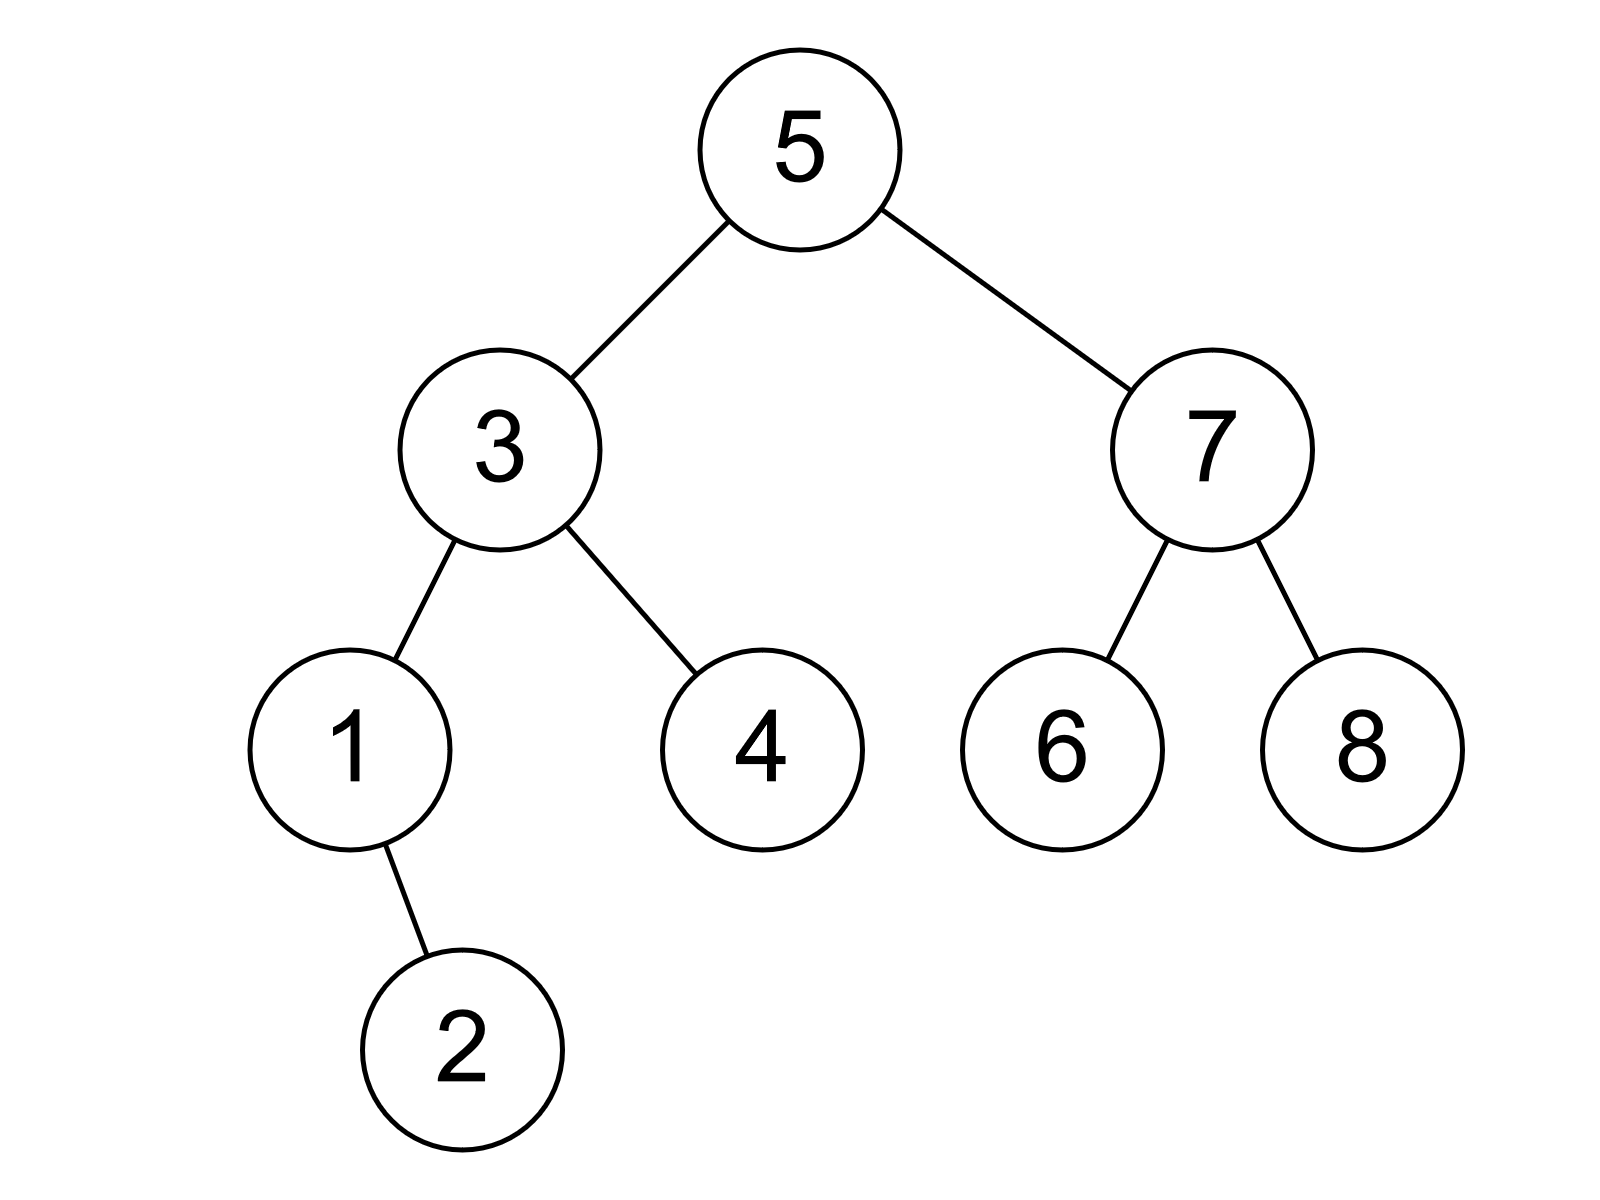
\includegraphics[width=0.22\textwidth]{img/1c}
        \end{figure}
        \FloatBarrier
        Wie viele Rechtsrotationen benötigen Sie?
        Zeigen Sie, dass Sie bei einem Suchbaum mit $n$ Knoten maximal $n - 1$ Rotationen benötigen, um den Baum in einen entarteten Baum zu konvertieren.
    \end{enumerate}
\end{aufgabe}

\begin{aufgabe}{2}{Rot-Schwarz-Bäume}
    \begin{enumerate}
        \item
        Nennen Sie zwei Vorteile und zwei Nachteile von RS-Bäumen in der Praxis im Vergleich zu AVL-Bäumen.

        \item Fügen Sie jeweils den Wert 7 in die folgenden RS-Bäume ein.
        Fügen Sie dafür einen roten Knoten mit Wert 7 an die entsprechende Stelle gemäß der Suchbaumeigenschaft in den Baum ein.
        Nutzen Sie anschließend jeweils die angegebenen Operationen, um alle RS-Baum-Eigenschaften wiederherzustellen.
        Wie sehen die Bäume am Ende aus?

        \begin{figure}[h!]
            \centering
            \begin{subfigure}[t]{0.3\textwidth}
                \centering
                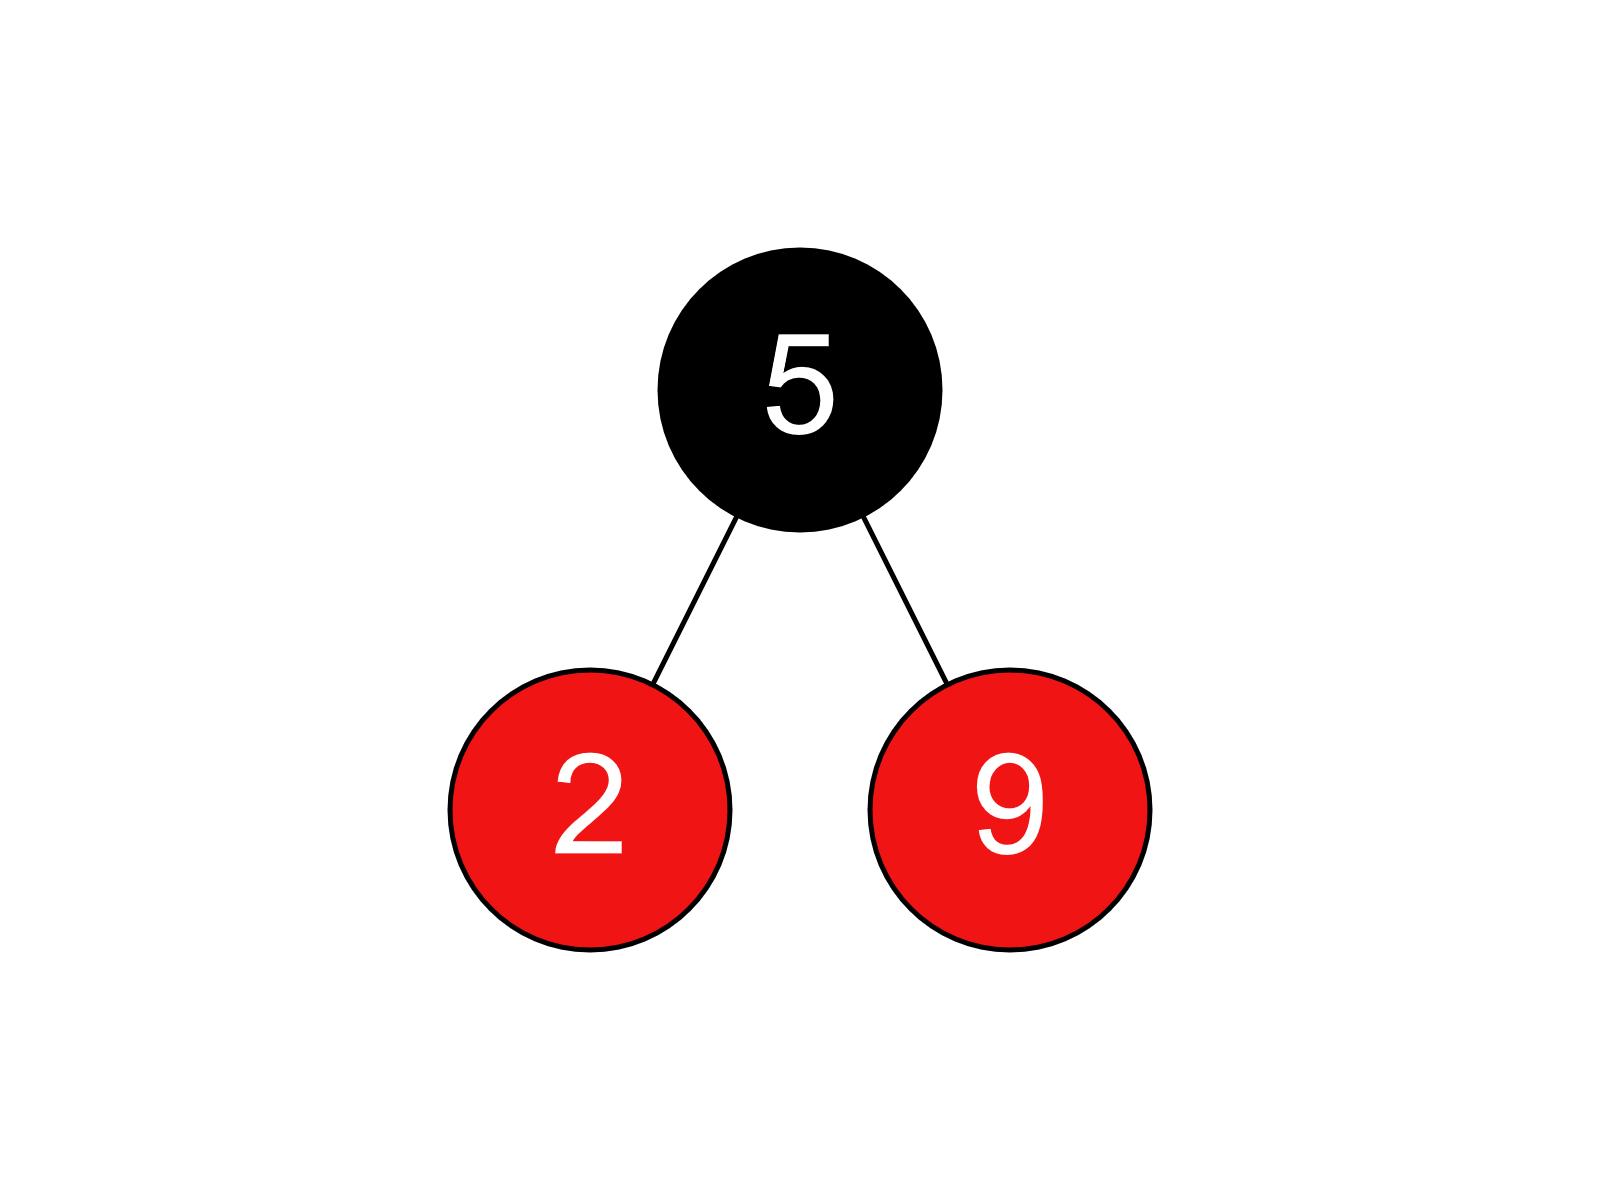
\includegraphics[width=0.6\textwidth]{img/2a_1}
                \caption*{i) Färbe 2 Knoten schwarz}
            \end{subfigure}
            \begin{subfigure}[t]{0.3\textwidth}
                \centering
                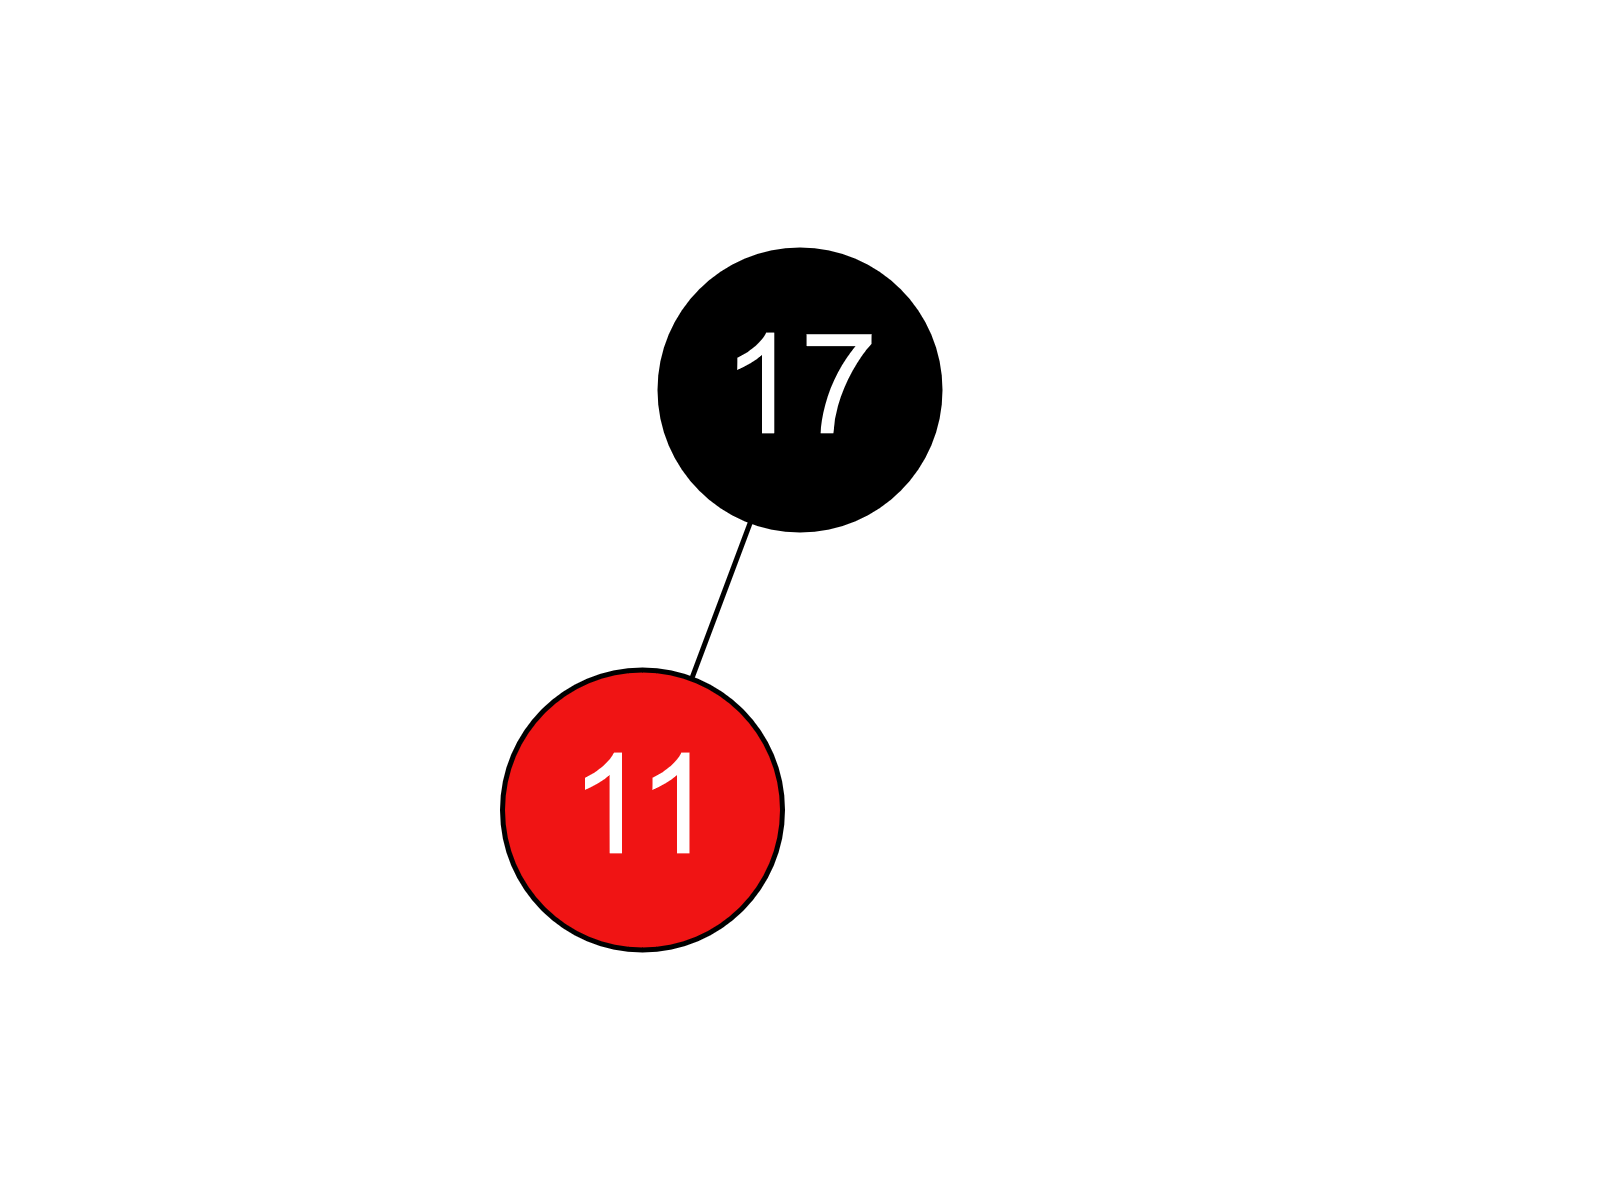
\includegraphics[width=0.6\textwidth]{img/2a_2}
                \caption*{ii) 1 Rotation, färbe 1 Knoten rot, färbe 1 Knoten schwarz}
            \end{subfigure}
            \begin{subfigure}[t]{0.3\textwidth}
                \centering
                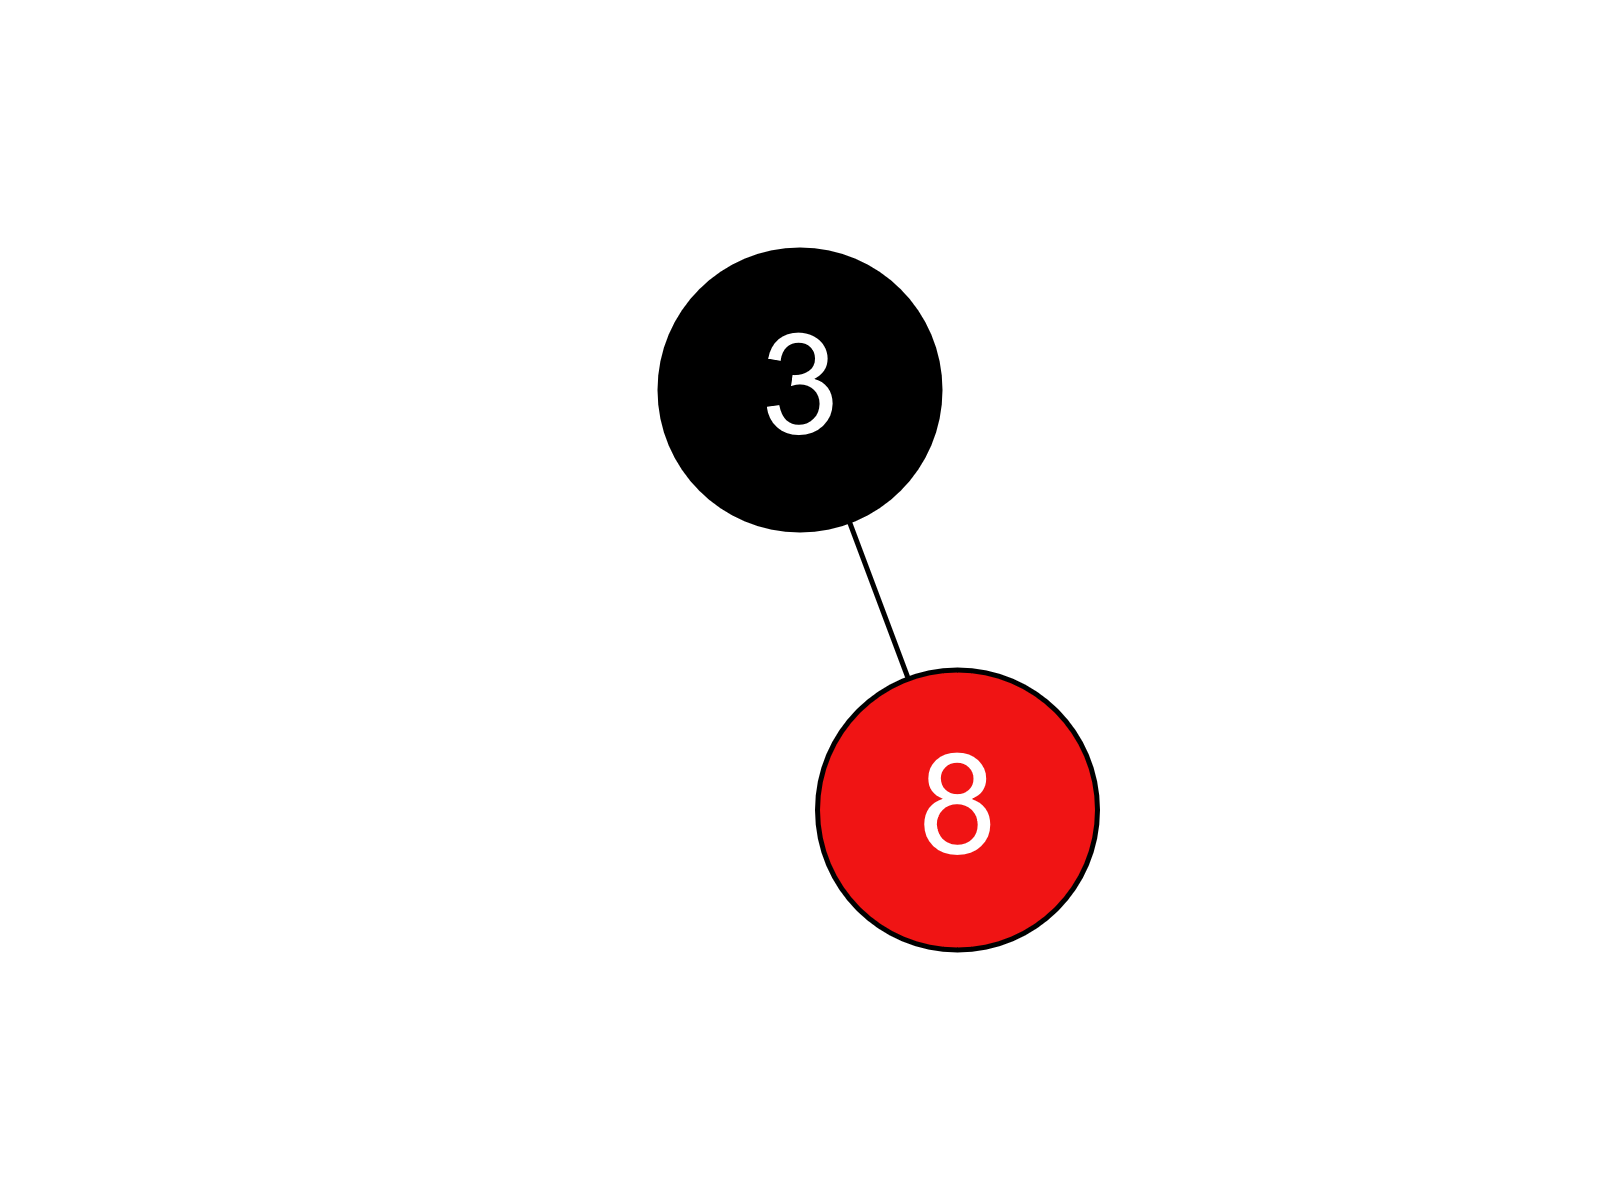
\includegraphics[width=0.6\textwidth]{img/2a_3}
                \caption*{iii) 2 Rotationen, färbe 1 Knoten rot, färbe 1 Knoten schwarz}
            \end{subfigure}
        \end{figure}
        \FloatBarrier

        \item Wie viele Werte sind in einem RS-Baum mit Schwarz-Höhe $k$ mindestens gespeichert? Wie viele maximal?

        \item Beweisen oder widerlegen Sie folgende Aussage: Bei jedem roten Knoten eines RS-Baumes sind entweder beide oder keiner der Nachfolger NIL.

        \item Wenn Sie in einem RS-Baum jeden schwarzen Knoten mit seinem/seinen roten Nachfolger(n) verschmelzen und die Nachfolger des roten Knotens als Nachfolger des schwarzen Knotens übernehmen, erhalten Sie einen Baum, mit potentiell mehr als einem Wert und mehr als zwei Nachfolgern pro Knoten.
        Beispiel:
        \begin{figure}[h!]
            \centering
            \begin{subfigure}[c]{0.2\textwidth}
                \centering
                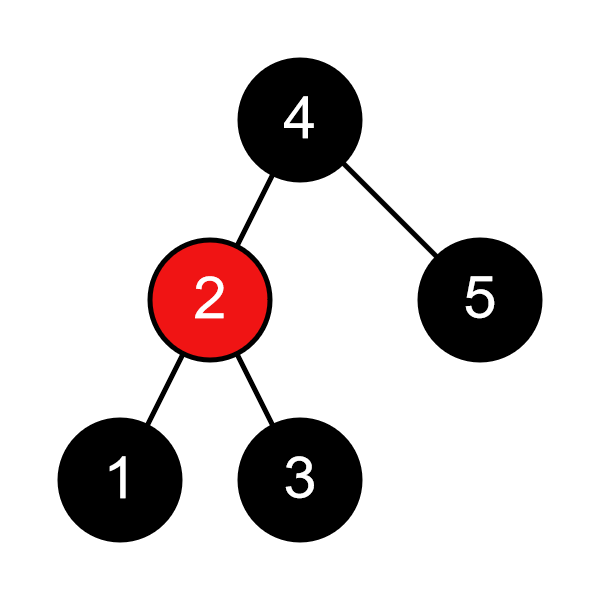
\includegraphics[width=0.8\textwidth]{img/2d_1}
            \end{subfigure}
            $\rightarrow$
            \begin{subfigure}[c]{0.2\textwidth}
                \centering
                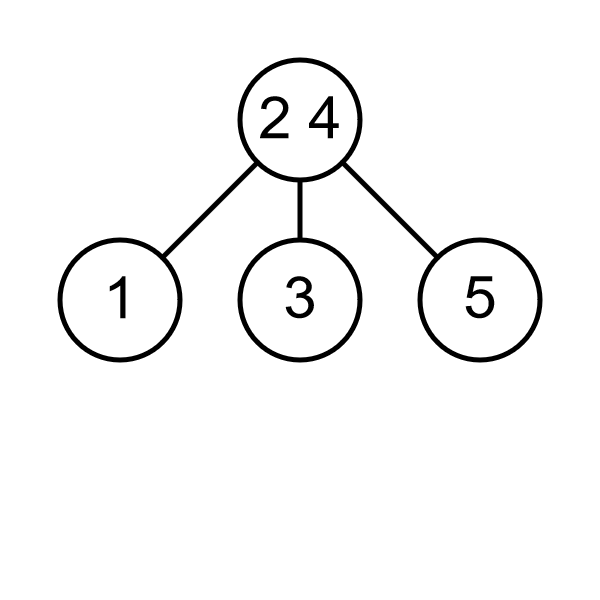
\includegraphics[width=0.8\textwidth]{img/2d_2}
            \end{subfigure}
        \end{figure}
        \FloatBarrier
        Welchen Baum erhalten Sie, wenn Sie beim folgendem RS-Baum jeden schwarzen Knoten mit seinem/seinen roten Nachfolger(n) verschmelzen?
        \begin{figure}[h!]
            \centering
            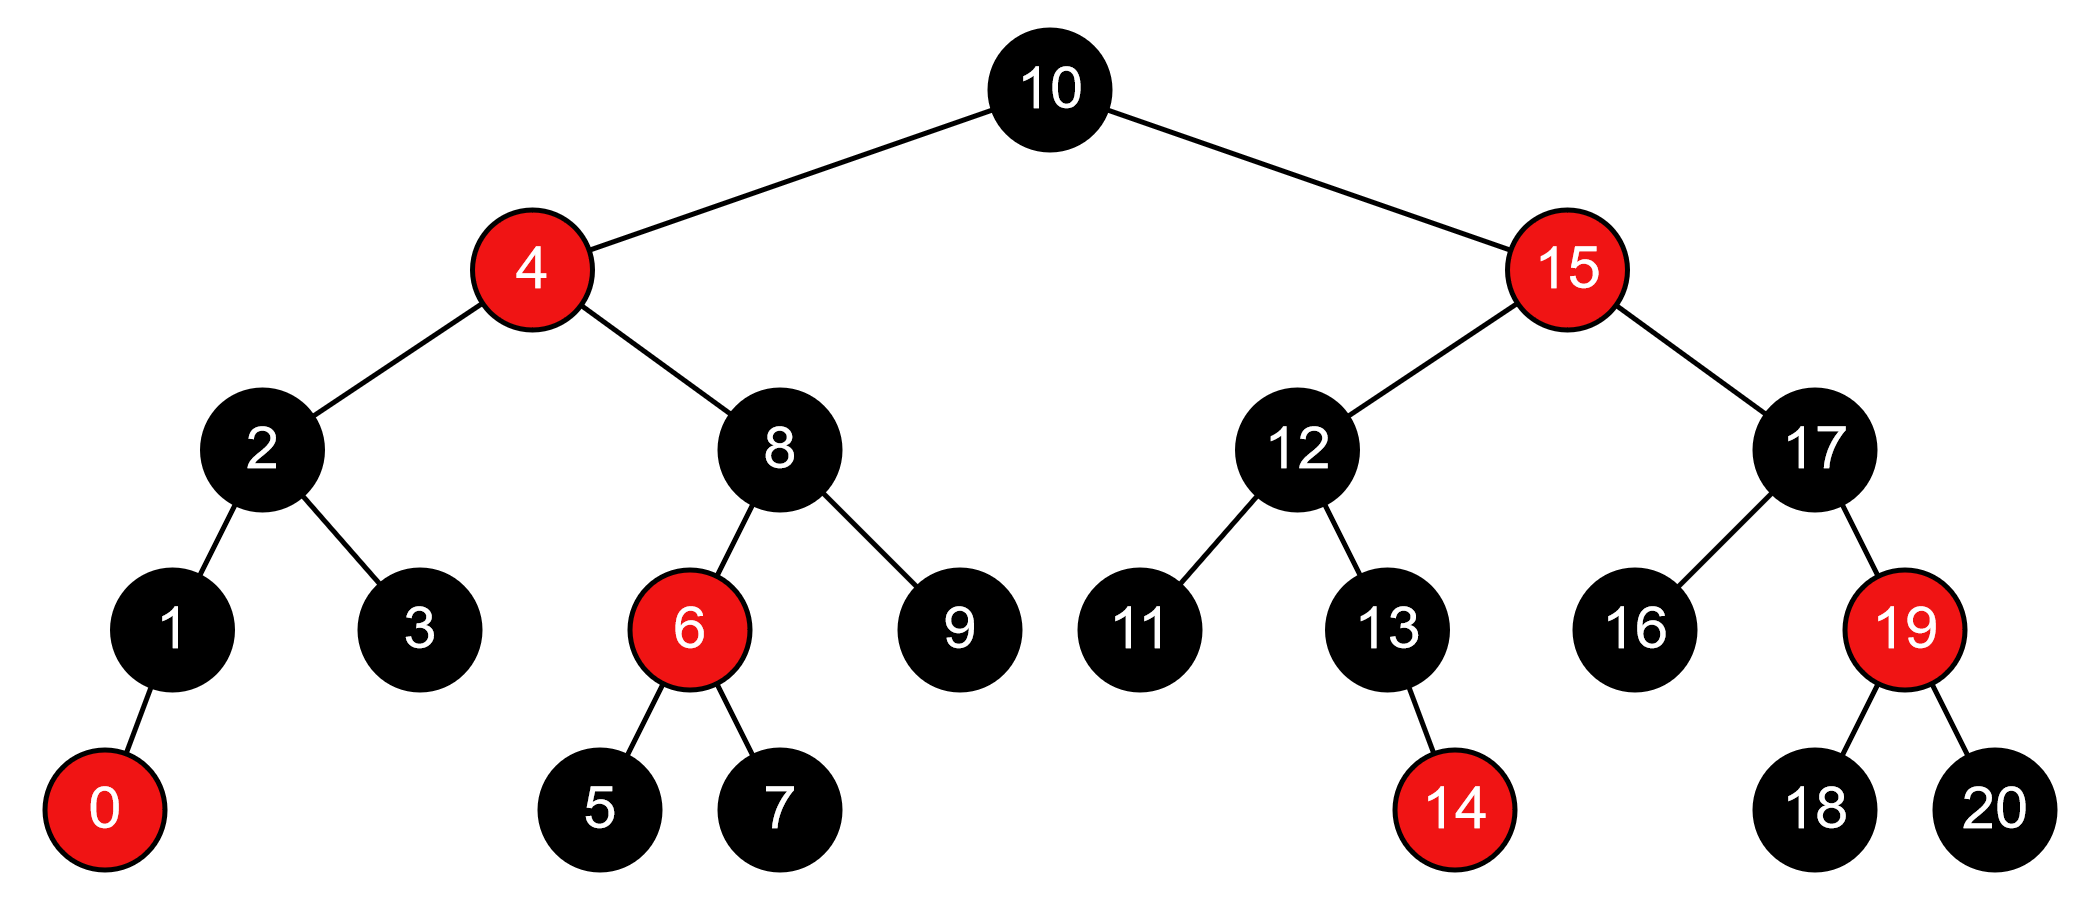
\includegraphics[width=0.5\textwidth]{img/2d}
        \end{figure}
        \FloatBarrier
        Welche Art von Bäumen erhalten Sie allgemein, wenn Sie die obige Transformation bei RS-Bäumen durchführen.
        Begründen Sie Ihre Antwort?
    \end{enumerate}
    
\end{aufgabe}

\begin{aufgabe}{3}{B-Bäume}
    \begin{enumerate}
        \item
        Nennen Sie zwei Vorteile und zwei Nachteile von B-Bäumen in der Praxis im Vergleich zu AVL-Bäumen.

        \item Geben Sie alle B-Bäume mit Ordnung 4 an, die die Werte 1, 3, 4, 5 und 7 enthalten.

        \item Gegeben sei ein leerer B-Baum der Ordnung 4. Fügen Sie sukzessiv folgende Elemente in den Baum ein: 
        7, 3, 8, 18, 10, 14, 12, 13, 6, 15, 20.

        \item
        Entfernen Sie aus dem resultierenden Baum der vorherigen Teilaufgabe folgende Elemente:
        3, 13, 6, 18, 20, 10.

        \item
        Gegeben sei folgender B-Baum der Ordnung 5 (Abbildung vorläufig):
        \begin{figure}[h!]
            \centering
            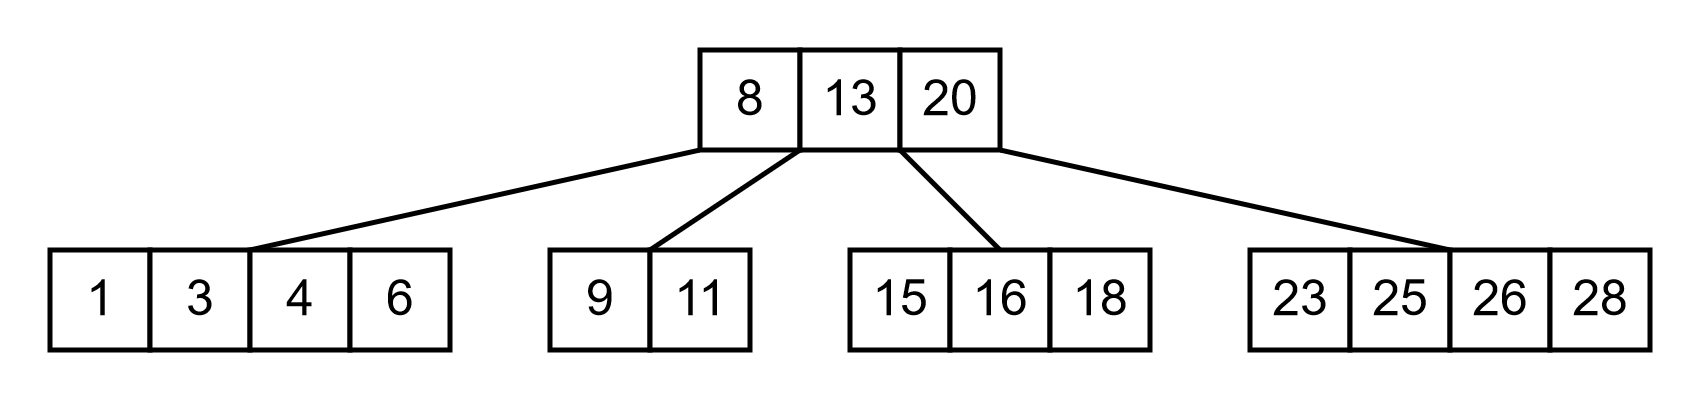
\includegraphics[width=0.5\textwidth]{img/3d}
        \end{figure}
        \FloatBarrier
        Führen Sie nacheinander folgende Operationen durch: 
        \textsc{Insert(2)}, \textsc{Remove(11)}, \textsc{Insert(7)}, \textsc{Insert(30)}, \textsc{Remove(8)}, \textsc{Remove(15)}.
        Geben Sie alle Zwischenschritte an.
        
        \item Angenommen, Sie haben einen B-Baum der Ordnung $t$ mit $n$ Werten im Arbeitsspeicher vorliegen:
        \begin{lstlisting}[language=c++]
class Node {
    int nSucc; bool isLeaf;
    int values[]; Node *succ[];
}
        \end{lstlisting}
        Implementieren Sie die Suchoperation, die überprüft, ob ein bestimmter Wert im Baum enthalten ist, in Pseudocode oder einer Programmiersprache Ihrer Wahl, einmal mit linearer Suche innerhalb eines Knotens und einmal mit binärer Suche.

        \item Geben Sie die Worst-Case-Laufzeiten der beiden Algorithmen der vorherigen Teilaufgabe abhängig von $t$ und $n$ an.
    \end{enumerate}
\end{aufgabe}

\end{document}